\documentclass[12pt]{article}

% Language setting
\usepackage[english]{babel}

% Page format
\usepackage[a4paper]{geometry}
\linespread{1.5} 

% Header
\usepackage{fancyhdr}
\addtolength{\headheight}{1.5cm} % make more space for the header
\pagestyle{fancyplain} % use fancy for all pages except chapter start
\fancyhf{} % clear header text chapter
\rhead{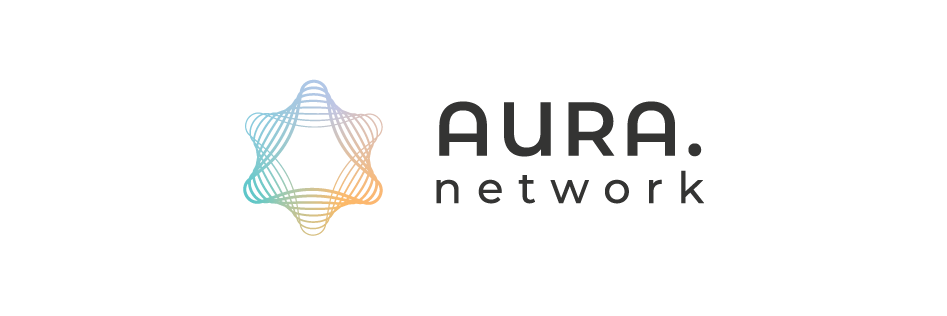
\includegraphics[height=1.3cm]{img/logo.png}} % right logo
\rfoot{\thepage}
\renewcommand{\headrulewidth}{0pt} % remove rule below header

% Useful packages
\usepackage{amsmath}
\usepackage{graphicx}
\usepackage[colorlinks=true, allcolors=blue]{hyperref}
\usepackage{draftwatermark}

% Fix too long hyperlinks in bibliography
\usepackage{url}
\def\UrlBreaks{\do\/\do-}

\title{Aura Network: a modern NFT-centric blockchain platform}
\author{admin@aura.network}
\date{\today}

\begin{document}
\maketitle

% \begin{abstract}
% Your abstract.
% \end{abstract}

\section{Context}

Cryptocurrencies (crypto) are becoming more and more popular by the day. Since the birth of Bitcoin in 2009, the crypto market has grown to thousands of billions US dollars in size. The success of crypto projects brings more innovations to the blockchain ecosystem. Recently, the hot topic of Non-Fungible Token (NFT) is an ideal case study of how blockchain technology is changing the world.

\subsection{NFT overview}
NFT origin can be traced back to the ERC-721 Ethereum token standard \cite{entriken2018erc}. A NFT is a distinguishable token that can be owned and transacted by individuals. 
Given an asset, either digitized or physical one, we can issue a NFT that embed the asset metadata including name, description and images to represent the ownership of the NFT creator to such asset. As this ownership relation can be freely traded in the market and the uniqueness property of the token, NFT investment is becoming widely popular. By the last quarter of 2021, the NFT sales world wide has surged to \$ 10.5 Billion \cite{nftsale}. Among the popularity of NFT, there are 6 main categories:

\begin{enumerate}
\item Collectibles: Due to the fact that NFT is unique, the possessions of special NFT is a natural demand for collectors. Some of the most well known NFT collectibles are CryptoPunks \cite{cryptopunks}, Bored Ape Yacht Club \cite{bayc}. Basically, any NFT can be considered collectibles. However, some have other usages in other categories as well. Currently, collectibles market value is at \$ 5.7 Billion, accounting for more than half of the whole NFT market.
\item Game: In-game assets can be represented as NFT. This unique interaction enables a new decentralized gaming trend of "play-to-earn" where players can obtain NFTs from the game then later sells it on the crypto market. Since May 2021, the Pokemon-inspired crypto game Axie Infinity \cite{axie} has rapidly gained attraction and currently provides one of the most valuable NFT collection in the world.
\item Art: Another form of collectibles NFT is digital art. NFT provides a new way for artists to increase the digital art value as it is truly unique. While the product itself can be easily copied, screen captured without permission, the origin of the art and it's owner cannot. The digital artwork "Everydays: the First 5000 Days" by Beeple is a collage of 5000 images created daily by the artist in the last 13 years \cite{beeple}. The work NFT was sold for \$69 million to a crypto investor in early 2021 and is the most expensive NFT to date. Besides traditional digital arts, website likes ArtBlock \cite{artblock} provides a programmable interface to allow artists to randomly generate unique images in their respective styles and tokenize them into NFTs. 
\item DeFi: As NFT is becoming valuable, its liquidity grows. Gradually, NFT is making its way into decentralized financial solutions. nftfi \cite {nftfi} offers a platform for NFT collateralise loans. Some NFT games like Cometh \cite{cometh} intelligently integrates token swap inside the token economy and gained a lot of attraction from the crypto community.  
\item Metaverse: with the rise of NFT and the recent announcements of big tech companies like Meta \cite{facebook}, Microsoft \cite{microsoft}, Metaverse NFT has gradually becoming the new trend of the crypto community. Pioneer projects such as Decentraland \cite{decentraland} and The Sandbox \cite{sandbox} allow users to create and share their own 3D objects with each other. These objects can be avatars, animal, land, real estate, etc. 
\item Other Utility: Outside of gaming, NFT can also be used for other utility purpose. Using Domain names NFT service like Ethereum Name Service \cite{ens}, users can register for ``.eth" Internet domains. VeeFriends \cite{vee} from Gary Vaynerchuk allows NFT holders to join Veecon, an exclusive conference for Gary community.
\end{enumerate}

\begin{figure}[ht]
\label{fig:nftsale}
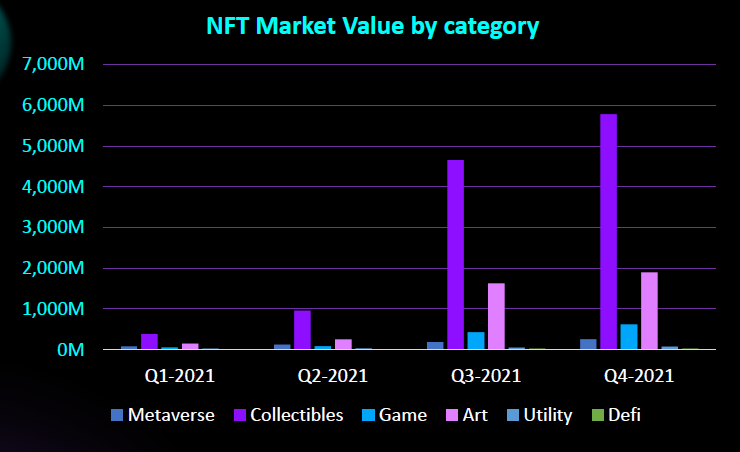
\includegraphics[width=14cm]{img/nftchart.png}
\centering
\caption{NFT Market value by categories in 2021 \cite{nftsale}}
\end{figure}

Figure \ref{fig:nftsale} shows the sale value of NFT in 2021 by these categories. We can see that most of the market value are around collectibles (\$ 5.7 Billion) and arts (\$ 1.9 Billion). While this is a good sign to show the appreciation for NFT and the accessible of the technology, we can expect more use cases for NFT in the future. NFT enables scarcity, uniqueness and proof of ownership to any unique asset in a decentralized way, not only digital items. Thus, they can be used to pretty much anything in the world, even in the physical world. 

\subsection{Challenges}
What will the future look like for NFT ? The technology is growing beyond simple collectibles or arts towards a much more diverse use of NFTs in finance, gaming, real estate, metaverse, etc. Every asset, digital or physical one, can have its own unique representation in the decentralized blockchain ecosystem and can be transacted without restriction. However, to enable that future, we will have to overcome several key challenges with the technology: usability, regulation and interoperability.

\emph{Usability} is a key factor to almost all software products that end users interact with. While NFT is just a token standard, the actual NFT object is owned, transacted by end users through various decentralized applications (DApps). Most of the current NFT scheme are based on Ethereum, thus they inherit drawbacks from the Ethereum network as well. The confirmation time is slow, Ethereum 1 has around 15-30 transaction per second (TPS), which is extremely slow for global scale DApps. Gas price is also extremely high especially when to mint new NFTs or upload metadata to the blockchain. Ethereum 1 carbon footprint is also very high due to the use of proof-of-work algorithm. These problems limit the utility of NFTs to use cases that concern only high value items rather than for everything. The tech community has been working actively in this problem for years. Ethereum 2 upgrade promises a more scalable and sustainable ecosystem. However, it is still a long way until all the upgrades are in place. Alternatively, other blockchains with much better usability are emerge. Flow is a new blockchain platform, originated from developers who built created CryptoKitties. Flow focuses on applications, games and digital assets. Binance Smart Chain (BSC) also supports NFT through the BEP-721 token standard. While non of the alternative choices is as popular as Ethereum, these blockchain platforms offer much better user experience and are more suitable for different use cases. 

Similar to any cryptocurrency scheme, \emph{regulation} is another major concern of NFT. Legally speaking, not all countries support the use and trade of NFT. Owning an NFT does not explicitly grant the owner any copyright or lawful enforcement over the real asset. Thus, investing serious tokens in NFT is not as easy as it look. For assets like books, arts, real life assets, they are taxable properties while their NFTs are not. It is unclear in the future whether NFT or any profit from NFT trading can be taxed or not.

Finally, there is little interoperability among different NFT ecosystems. There is currently no way to directly transmit an NFT from Ethereum to BSC yet. While cross-chain communications are blooming, it is still some time before we can see all of these advancements work with NFT. While the major NFT schemes are concentrated in Ethereum, this problem prevents the wide adoption of the technology to other blockchain platform.

\section{Introducing Aura Network}
Given all of the challenges above, we introduce \emph{Aura Network}, a NFT-centric blockchain platform that focus on expanding the use of NFT across various industries. Our vision is to create an one-stop destination for minting, evaluating, querying and transacting NFT, to become a pioneer NFT infrastructure for the future. Aura Network focuses on solving the 3 challenges of \emph{usability}, \emph{regulation} and \emph{interoperability} of the current NFT market.

This section provides a high level view of 3 main aspects of Aura Network: an universal framework for managing NFT, a multi-chain solution to expand the use of NFT and a NFT infrastructure for the metaverse.

\subsection{Universal framework for NFT}
The original token standard ERC-721 and ERC-1155 laid a foundation for NFT standard interfaces. However, how these tokens are created and used in DApps are not standardized yet. This allows developers to have more room for creativity. Wang et al. \cite{wang2021non} summarized two popular protocols for managing NFT in DApps:
\begin{enumerate}
\item \textbf{Top to Bottom:} where an owner creates the asset, mints the NFT token that represent the asset and trade it with others through the $transferFrom$ function. This pattern is used in CryptoPunks \cite{cryptopunks}, Beeple's Everydays \cite{beeple}, etc.
\item \textbf{Bottom to Top:} where the DApp creates a NFT template that allows users to invoke and create their own unique NFT based on that template. This is used in platform generated NFT such as artblock \cite{artblock} and NFT game like Axie Infinity \cite{axie}.
\end{enumerate}

Most of the functions from these two protocols are concerning either the NFT creator and buyer. There might be other stake holders in the protocol such as the DApp creator and the exchange marketplace. These are suitable for simple digital items and simple use cases. However, if we are targeting a vastly broad NFT market that involve not only collectibles and digital items but also physical assets, comprehensive digital contracts, etc., there are more parties involve. We now give an example of possible important stakeholders that may appear in such market:

\begin{enumerate}
    \item \textbf{Custodian:} Similar to the term in banking, a custodian bank is a financial service provider that hold customer's assets for safekeeping. While "Not your keys, not your coins" is widely accepted in the blockchain community, Coinbase and various banks around the world are offering high quality custodian services for crypto assets. They provide cold storage, security controls and even insurance plan for protecting cryptocurrencies. This practice is also long established for physical assets as well. Keeping authorized papers, will or high value items like jewels, antiques are very common for custodian services.
    
    To NFT users, custodians can offer safekeeping physical items in their safe vaults and only allow user to redeem those items if they own the NFT. If NFT provides a way to prove the ownership of an asset, we can also expect custodian to prove that they are, in deed, holding the corresponding physical item in their safe vaults by an on-chain transaction.
    
    \item \textbf{Auditor:} In finance, an auditor refers to the person that is authorized to verify the correctness of financial documents and whether they comply with regulation. In security, auditors conduct reviews and make sure the system is protected from common threats. In a lot of case, the asset owner, buyer or the exchange do a part of the auditor job such as KYC, proving the legitimacy of papers with records, bills, etc. However, in the case of issuing NFT for high value items like real estate, having a third party auditor brought in to certify the legitimacy of the asset as well as the right to sell of the owner will definitely increase the trust of the buyer and value of the item.
    
    \item \textbf{Evaluator:} In the real estate industry, property or land valuation is often a required procedure to give an estimation of market value to the property. Diamonds are evaluated based on their quality factors in clarity, color, cut, and Carat Weight. The valuation process mostly conducted professionally and can give a relatively correct value of an asset rather than subjective opinion. Similarly, NFTs of valuable assets can also be evaluated in a lot of criteria: the origin of the asset, level of granted permission, market price of similar items or depending on the utility of the NFT.
    
    \item \textbf{Asset Manager:} With items that have high utility such as cars, real estate, a local manager who keep tracks of utility usage of the item greatly benefits the community. Real estate companies often have house managing companies to do house maintenance, screening tenants or collecting rents. If NFT can represent the ownership of a real estate, the NFT owner not only should have all documentations relating to the properties, but also can get local asset managers on board to do all the manual work for them later on. 
    
    \item \textbf{Investor:} Another new use case of NFT is to fractionize the NFT to allow multiple investors to co-invest in the item. This fractional ownership adds new ways for integrating NFT with DeFi scheme such as Uniswap as each fraction is fungible. Thus, multiple investors can pool up and join the NFT investment game.
\end{enumerate}

Custodian, auditor, evaluator, asset manager and investors are just some sample of possible stakeholders that are needed in the NFT market. We have seen some use cases that require those parties. However, a complete platform that allows all of them to work together on-chain is unheard. This is why we create Aura Network. We envisioned Aura Network to be a one stop destination for all stakeholders and projects in the NFT ecosystem. Every interaction with NFT and its counterpart in the physical world should be reflected on-chain.

\subsection{Connecting to other Blockchains}

With the success of Bitcoin, Ethereum, Cardano and others, a lot of crypto project was born, creating many isolated blockchain networks. With multiple blockchains coexisting, cross-chain communication solutions emerge. Atomic swap, cross chain messages are all examples of the capability to link different blockchains together to create a more cohesive ecosystem that benefits everyone. However, at the moment, there is not yet a mainstream solution for either moving a NFT from one blockchain to another, or having multiple NFT on multiple blockchains that represent the same asset. While this is mostly due to the poor interoperability among different blockchain platforms, we can expect that this issue can be resolved in the near future due to the advancement of cross-chain bridges similar to XP.Network \cite{xpnetwork} or related projects. 

Another part of blockchain community that we need to look at is the private blockchain sector. Standing beside the success of crypto projects, private blockchain projects are slowly gaining attractions. Private, consortium or permissioned blockchain often refer to systems that consist of one or several authorized parties that create a blockchain network for specific business purposes. Imagine a group of companies who want to create a distributed network for transparently exchanging assets, tracking items or sharing documents. Unlike its counterpart, private blockchain is more appealing for companies, enterprises or governments as they are easier to control and do not require volatile currencies to operate. Success of the crypto trend in 2020 also brought a lot of opportunities to private blockchain eco-system. The private blockchain sector is predicted to generate \$176 Billion in 2025 then surge to  \$ 3.1 Trillion in business value by 2030 \cite{privatebc}. 

Can NFT become a game changing use case in private blockchain ? a lot of businesses are looking into loyalty, insurance or traceability use cases where the blockchain ledger is an immutable storage of important data. This fits the idea of NFT very well. However, there isn't any mainstream use case that can bring NFT to the private blockchain sector. Typically, enterprises or businesses are main adopters of private blockchain as they  require more control over the network. By having a bridge to public blockchain and vice versa, NFTs defined on Ethereum, BSC and other networks can be moved to private chains, where they have more utility in dealing with real world problems that businesses are dealing with in their private blockchain setup. In turn, by having a route to the public side, businesses now have access to a market of millions users and billions USD worth of values circulating every day. This increases liquidity on private networks massively and enables many other use cases that a single blockchain network can not achieve.

This is the second aspect that Aura Network is trying to solve. The Aura blockchain platform should be capable of bridging to other blockchain network, either public or private ones and vice versa. Thus, NFT owners can bring their on0chain assets to any place, any app, at any time. 

\subsection{Towards the metaverse}
In this last section, we look at the recently popular trend of ``metaverse". The word is a combination of ``meta" and ``universe". It describes a hypothetical virtual world that is linked to the physical world. The term was coined in a science fiction novel \emph{Snow Crash} by Neal Stephenson in 1992. While the concept of virtual world is not new as computer games has been around for decades, the metaverse concept brings more integration between virtual and physical world. In the metaverse, users are represented as \emph{Avatars} and through them, they can interact with the digital environment which is a metaphor of the real world \cite{lee2021all}.

While the term \emph{metaverse} was coined in 1992, the development of the idea was dated way before it. The table top game \emph{Dungeon \& Dragons} was published in 1974, allowing players to submerge in a fantasy medieval European theme world with super powers and mythical creatures. That was more than a decade when the first personal computer was introduced. Later on, with the booming of the Internet, the table top imaginative world then become virtual, digital world of massively multiplayer online games (MMOG) such as \emph{Second Life}, \emph{Minecraft}. Players then can also have a mix experience of the virtual and physical world through games like \emph{Pokemon Go} and extended reality hardware devices like \emph{Hololens} or \emph{Oculus Rift}. Blockchain based Metaverse came later. The NFT game \emph{Crypto Kitties} in 2017 is the first popular blockchain game that allows players to truly own in-game assets and create a new blockchain based virtual economy. Following the kitties, other games like \emph{Decentraland}, \emph{The Sandbox}, etc. are creating new opportunities for players to not only submerge into the metaverse world, but also actually own some part of it themselves.

The metaverse is more than just games. Lee et al \cite{lee2021all} show us the three steps of evolution in technology that support metaverse. The first step of \emph{Digital Twins} is where physical objects can be projected to their digital form. Photos, 3D models are the examples. Next step is \emph{Digital Natives} where users can freely create new content, virtual object that are based on the projected ones. User can own it, sell it in a decentralized manner, etc. This is already achieved in NFT games. Finally the last one, \emph{Co-existence} is where both physical and digital objects exists, are linked together and users can interact with both. This is the step that Aura Network wants to aim for.   

\begin{figure}[ht]
\label{fig:metaverse}
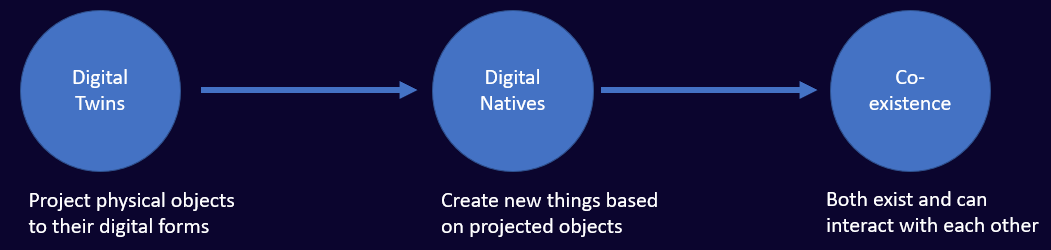
\includegraphics[width=14cm]{img/metaverse.png}
\centering
\caption{Evolution states of metaverse \cite{lee2021all}}
\end{figure}

Mapping real world, physical asset to NFT is an important step in achieving the co-existence state of the metaverse. As an universal framework for working with NFT, Aura Network final step is to work with games and service providers like Decentraland, Axie Infity, Meta, Microsoft, etc. to bring NFT on chain to these virtual world.

\section{Architecture}
In this section, we will present the high level software architecture of the Aura Network ecosystem. Particularly, we will first go through the architecture of the Aura Blockchain platform. Next is the envisioned eco-system that we will build on top of the platform and finally, we give an overview of a complete hypothetical use case of mapping real life assets on the Aura Network.

\subsection{Blockchain Platform}
The Aura Network Blockchain platform is a \emph{Layer-1 blockchain} built using \emph{Cosmos SDK} \cite{kwon2019cosmos}. The Cosmos SDK is an open-source framework for building proof-of-stake blockchains. It allow developers to create a blockchain platform from scratch with native interoperate capability with other blockchain platforms. 

\begin{figure}[ht]
\label{fig:architecture}
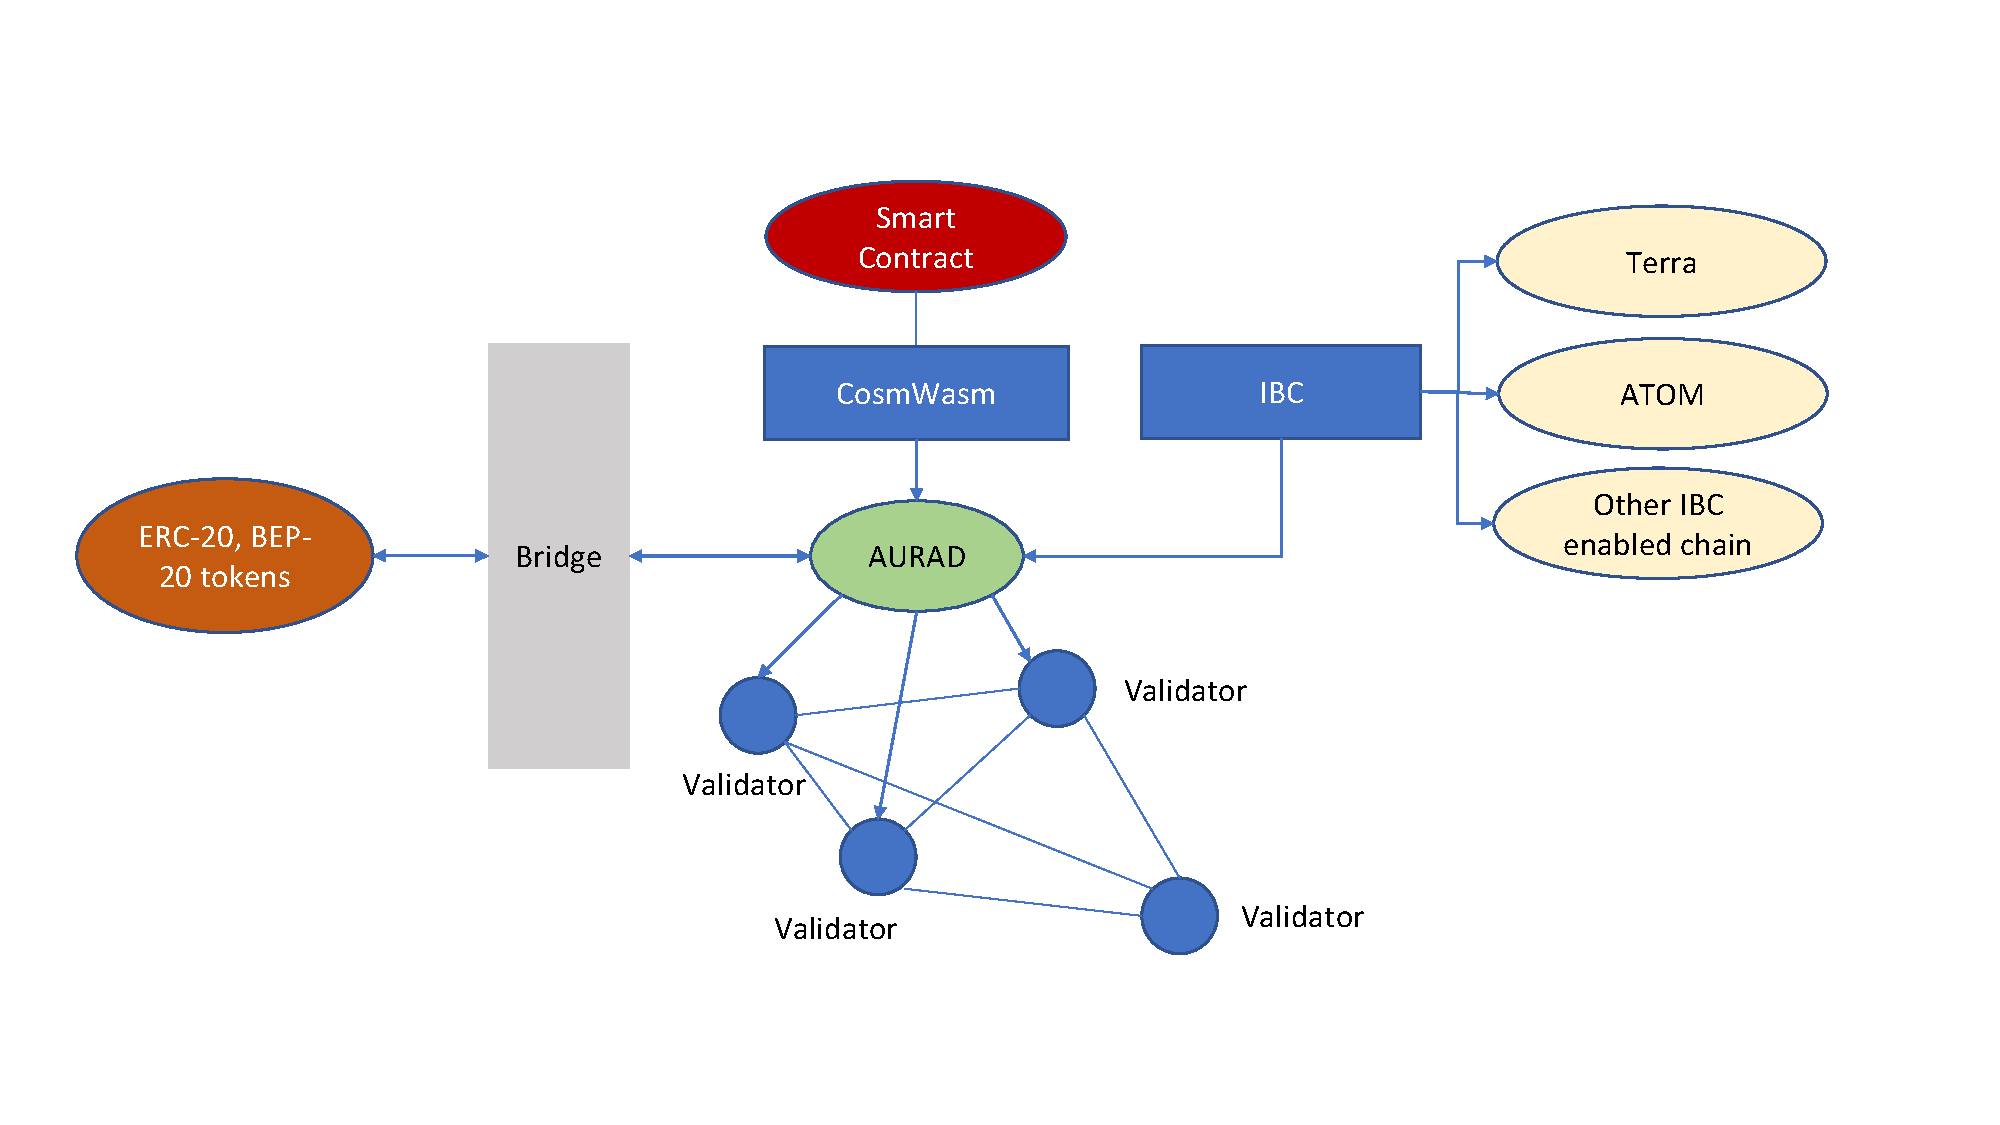
\includegraphics[width=\textwidth, trim={5cm 2cm 5cm 0}, clip]{img/architecture.pdf}
\centering
\caption{The Aura Network blockchain platform architecture}
\end{figure}

Figure \ref{fig:architecture} shows the high level architecture of the Aura blockchain platform. There are several main components that we want to highlight in this architecture:

\subsubsection*{Validator}
\emph{Validators} are blockchain nodes that participate in the consensus process to confirm transactions and producing blocks.
The consensus engine is \emph{Tendermint}~\cite{buchman2016tendermint}, a Byzantine Fault Tolerance state machine replication engine while he Proof-of-Stake (PoS) logic layer is provided by the Cosmos SDK. 

\subsubsection*{aurad}
\emph{aurad}, short form of ``Aura Daemon" refers to the compiled platform binary that runs on all Validator nodes. The  

\subsection{Eco System}
\begin{figure}[ht]
\label{fig:auraeco}
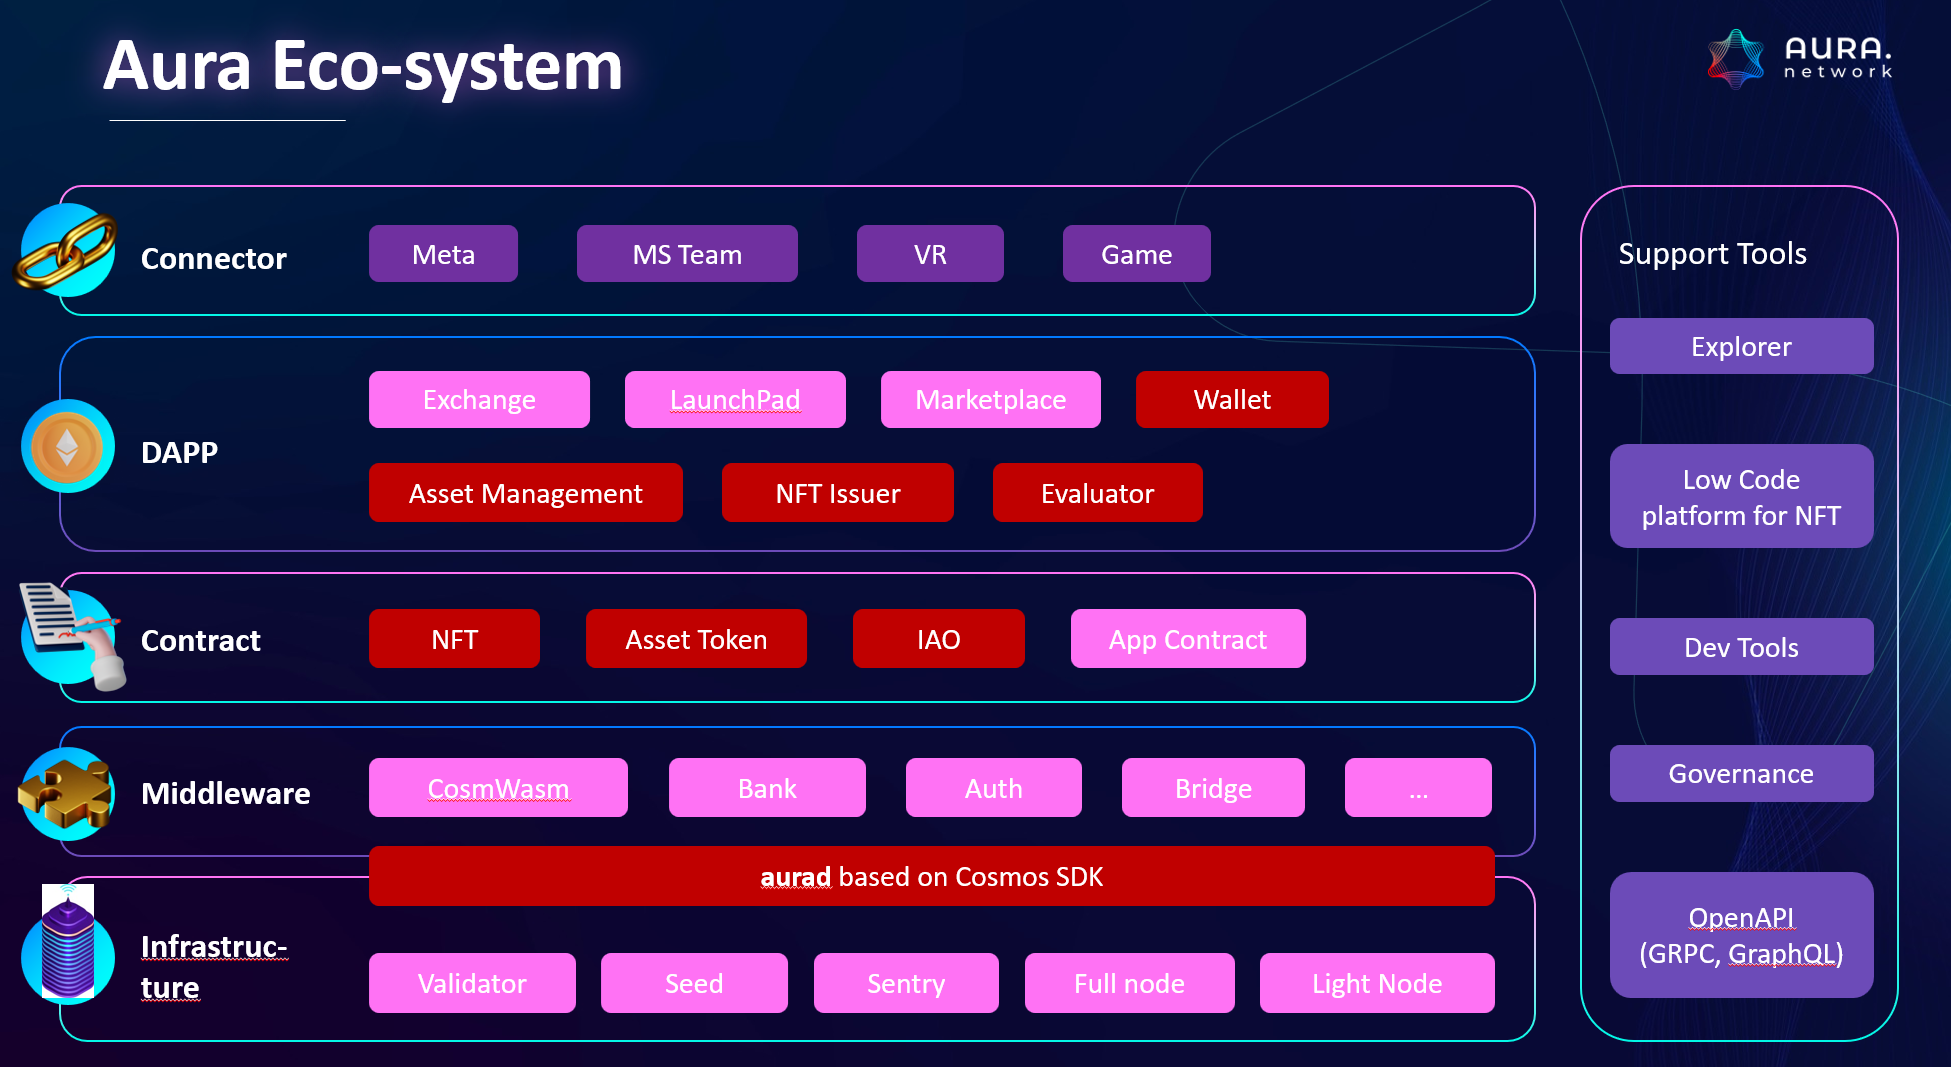
\includegraphics[width=14cm]{img/auraeco.png}
\centering
\caption{The Aura eco-system}
\end{figure}

\subsection{Mapping Real life Assets}


\section{Tokenomics}

\section{Roadmap}

\bibliographystyle{plain}
\bibliography{references}

\end{document}